%%%%%%%%%%%%%%%%%%%%%%%%%%%%%%%%%%%%%%%%%%%%%%%%%%%%%%%%%%%%%%%%%%%%%%%%%%%%%%%%%%%%%%%%%%%
%                               Evaluation - 16pp
%%%%%%%%%%%%%%%%%%%%%%%%%%%%%%%%%%%%%%%%%%%%%%%%%%%%%%%%%%%%%%%%%%%%%%%%%%%%%%%%%%%%%%%%%%%
\chapter{Evaluation}
\label{sec:evaluation}

\section*{Summary}
%To evaluate our approach we plan to run several experimental tests within a group of, at least, ten subjects. 
%With these experiments we want to obtain statistical measures about our approach and be able to conclude 
%on which combinations of feedback could have better performance in guiding a patient.

%We will be using two different experiments in order to achieve comparable results. 
%The first experiment will consist of a \ac{PT} and a test subject. 
%The \ac{PT} will demonstrate a given exercise to the test subject and then evaluate their execution without giving any kind of feedback. 

%The second experiment will involve guiding a test subject through the same exercise as the first experiment, 
%using different combinations of visual, audio and haptic feedback.
%The resulting performance will be analyzed and several data gathered. 
%We will take into account the following metrics, (a) the trajectory error between the Exercise Model and 
%the patient's actual execution, (b) the time it takes for the patient to finish the exercise 
%and (c) the time it takes for the patient to recover to the correct position if mistaken.

%We will start by using a unimodal approach, to obtain measurements using only one of the 
%available feedback modes each time. After the unimodal experiments, we will begin the multimodal 
%approach experiments by combining the available feedback and repeat the same measurements previously done.

%Even though our main focus is to provide concurrent feedback (during the execution), its frequency will be altered in order to evaluate the patient response. Therefore, further in the end, we will provide only terminal feedback (without guiding cues during the execution) to analyze if the patient successfully learned the movement.

For the evaluation of the SleeveAR, we intended to observe how well a subject recreates simple arm movements just by following the feedback at his disposal. 

Since tests involve executing simple arm movements, five different exercises were created for this evaluation. \todo{colocar links de youtube?} These exercises were simultaneously recorded both by video and by the SleeveAR's Learning Architecture. This way, we guarantee the same movement is being stored in video and in our system.

This chapter presents a detailed description of the experimental tests. It addresses the experimental methodology employed for testing our prototype with test subjects, the category of performed tests, the measurement metrics, and the characteristics of the collected sensor information. It also presents the experimental results and their critical analysis. All the results will be discussed in order to achieve a better understanding about our prototype functionality and performance.
Finally, the chapter reports some of the most important critics elaborated by a professional physical therapist after using our system.

\section{Methodology} \label{evaluation-methodology}

\begin{table}
\centering
\begin{tabular}{lll}
\hline
\multicolumn{1}{|l|}{\#}& \multicolumn{1}{l|}{Stage}         & \multicolumn{1}{l|}{Time}       \\ \hline
\multicolumn{1}{|l|}{1} & \multicolumn{1}{l|}{Introduction}  & \multicolumn{1}{l|}{2 minutes}  \\ \hline
\multicolumn{1}{|l|}{2} & \multicolumn{1}{l|}{SleeveAr}      & \multicolumn{1}{l|}{15 minutes} \\ \hline
\multicolumn{1}{|l|}{3} & \multicolumn{1}{l|}{Video}         & \multicolumn{1}{l|}{10 minutes} \\ \hline
\multicolumn{1}{|l|}{4} & \multicolumn{1}{l|}{Questionnaire} & \multicolumn{1}{l|}{3 minutes}  \\ \hline
\end{tabular}
\caption{SleeveAR evaluation stages}
\label{table:teststages}
\end{table}

%\begin{itemize}
%\item divided by 3 main parts
%\item executing movements following video instructions
%\item executing movements following SleeveAR
%\item answering a small form at the end
%\end{itemize}

This section describes the experimental methodologies for testing our prototype. Each participant followed this methodology in a similar way.

The average time spent with each participant was approximately thirty minutes. As we can observe in Table \ref{table:teststages}, the test was composed of four stages:

\begin{enumerate}
\item \textbf{Introduction}

Before the actual test, participants received a brief explanation concerning the main goal of our thesis. They were also made aware of what would the full experimental test consist of.

\item \textbf{SleeveAR}

The participant executes the exercises, as described in section \ref{evaluation-tasks}, while following our prototype real-time feedback.

\item \textbf{Video}

For each of the five exercises selected for this evaluation, the participant  watches a video of its execution at least two times. Then, while following the video playing, the participant executes the same movement based on the video observation.

\item \textbf{Questionnaire}

Finally, a small questionnaire should be filled by the participant. This questionnaire includes questions concerning stage 2 and 3, while also providing us some information about the user's profile.

\todo{Artur: Questionnaire in Annex?
JV: Yes, we still did not include the questionnaire, I'll take care of it in the afternoon}

\end{enumerate}

In order to gather data for further result analysis, each execution of an exercise generated a Log with all the necessary information about the participant's movement. \todo{descrever Logs mais detalhadamente}

Even though we are presenting this ordering for the four stages, half of the participants started by doing the third stage before the second, for the purpose of obtaining a more balanced sample of results.

\section{Performed Tasks} \label{evaluation-tasks}
The same five exercises were executed for both the above mentioned second and third stages.

Each exercise was simultaneously recorded with a video camera and with motion tracking devices. Under these circumstances, we made sure that the content being stored in video format directly represented the data being stored on SleeveAR's architecture.
The tasks performed in stage 2 and 3 had the identical goal of recreating the five recorded exercises.

\todo{explicar como era cada exercicio? Sim}

\section{Environment and Participants} 



\section{Results}
\label{sec:results}

The empirical evaluation addressed the correctness of the executed exercises. Experiments with test subjects were performed for a baseline scenario, consisting of exercise execution through video observation, and for a patient assisted scenario consisting of real-time feedback provided the proposed prototype. The performance metrics is given by the degree of similarity between the participants' arm trajectories and the original trajectories demonstrated by the therapist. It is measured using the \textbf{\ac{DTW}} \todo{referencia para o algoritmo} algorithm, 
which is appropriate for measuring a degree of similarity between two temporal sequences which may vary in time or speed. With the application of this algorithm in mind, the recorded movements can be reformulated as a sequence of positions. One can then compare the performance values for both the proposed solution and the baseline scenario.

Due to an arm movement being divided by the upper and fore arm sections, the \ac{DTW} was applied to each individually, thus providing us with a more detailed set of values. This separation enables to observe if there were significant performance differences between each arm region.

The final \ac{DTW} values of each exercise are the result of adding both arm regions' DTW values. It is important to highlight that with the following results, DTW values closer to zero directly represent movements more similar to those of the original demonstration.

\todo{arredonda os numeros, maximo 3 casas decimais e.g. 0.090 e 0.165}

For the first exercise, we can observe in Figure \ref{fig:sleevearVSvideoEx1} the test results from all participants, both using the SleeveAr and by observing the respective video.
These results clearly show SleeveAR provided a higher similarity when comparing to the original exercise. 
In terms of statistic values, participantes achieved an average \ac{DTW} value of \textbf{0.114181315} and a Standard Deviation of \textbf{0.090349091} when using SleeveAR.
On the other hand, an average \ac{DTW} value of \textbf{0.438959688} and a standard deviation of \textbf{0.164684962} was achieved when relying on video observation. 
Based on these results, in the first exercise, SleeveAR clearly improve participant's performance which were able to re-create the original exercise better then by video observation. 

Based on evidence from the experimental results, similar conclusions can be drawn for the other four exercises. Table \ref{table:dtwavg} presents the average DTW and standard deviation for all five exercises \todo{aqui mudar para grafico em vez de tabela}

\begin{figure}[t!]
    \centering
    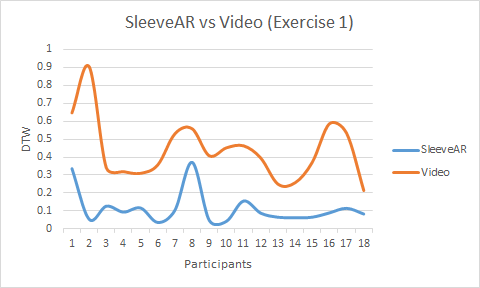
\includegraphics{imgs/results/sleevearVSvideoEx1.png}
    \caption{Exercise 1 DTW comparison between SleeveAR and observing video.}
    \label{fig:sleevearVSvideoEx1}
\end{figure}



\begin{table}
\centering
\begin{tabular}{c|c|c|c|c|c|}
\cline{2-6}
\multicolumn{1}{l|}{}                               & \multicolumn{5}{c|}{Exercises}             \\ \cline{2-6} 
                                                    & 1      & 2      & 3      & 4      & 5      \\ \hline
\multicolumn{1}{|c|}{SleeveAR Average DTW}          & 0.1142 & 0.1472 & 0.3262 & 0.1289 & 0.3801 \\ \hline
\multicolumn{1}{|c|}{Std Dev}                       & 0.0903 & 0.148  & 0.2005 & 0.0595 & 0.2762 \\ \hline
\multicolumn{1}{|c|}{Video Observation DTW Average} & 0.439  & 0.263  & 0.3549 & 0.1945 & 0.2733 \\ \hline
\multicolumn{1}{|c|}{Std Dev}                       & 0.1647 & 0.0921 & 0.1697 & 0.0657 & 0.0887 \\ \hline
\end{tabular}
\caption{My caption}
\label{table:dtwavg}
\end{table}

\begin{figure}[t!]
    \centering
    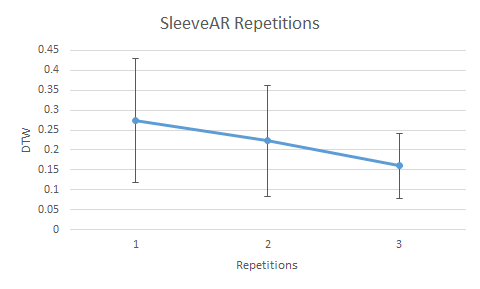
\includegraphics{imgs/results/dtw_repetitions.png}
    \caption{DTW value variation with each repetition using SleeveAR.}
    \label{fig:dtw_repetitions}
\end{figure}

Focusing solely on SleeveAR results, figure \ref{fig:dtw_repetitions} presents the average DTW on each of the three trials executed by participants for each exercise. 

\todo{in methodology, say that there are three trials}

These results clearly show an improvement on a patient's performance in just a small number of repetitions. 
Not only the average DTW values become smaller, i.e. closer to the original, with the number of repetitions, but also the standard deviation appears to diminish. 
Indeed, with each repetition, the participant is able to see where he failed the most \todo{falar na implementation sobre a session review}. Hence,
the system enables improvements on user's next repetition.

\todo{There is no time for this until delivery, but for your knowledge: we could now conduct a hypothesis t-test (test statistic follows a Student's t-distribution) on the slope of the regression line Y = Β0 + Β1X, where Β0 is a constant, Β1 is the slope (regression coefficient), X is the noise and Y the execution time value. If there is a significant linear relationship between these two variables, the slope Β1 will not equal zero. Hence, the hypothesis to evaluate is
- H0: Β1 = K. The null hypothesis states that the slope is equal to K (K = 0)
- Ha: Β1 ≠ K. The alternative hypothesis states that the slope is not equal to 0}

\section{Validation with Physical Therapist}

A professional physical therapist, besides the test subjects, also tested the SleeveAR prototype, performing the same exercises as the evaluation ones performed by the test subjects. This expert feedback was afterwards gathered in an interview as a qualitative evaluation of the proposed solution.

First of all, this prototype main vision was to prove we were able to guide subjects through pre-recorded exercises, so the latter were as close as possible of the original exercises. With this in mind, we wanted to evaluate the usefulness of this tool in a regular physical therapy work environment. We also wanted to understand what would be missing to make SleeveAR a more complete tool for a common use along this field of rehabilitation.

We will now present the most significant feedback, stressing both the positive and negative aspects of the proposed solution.


\begin{itemize}
\item \textbf{Missing feedback from one of the three axis}

A fully complete SleeveAR real-time feedback would need to take into account the missing axis of movement. Since this prototype focused on guiding the arm through relatively simple movements, we had not previously detected this problem. But, consequently, in the evaluation tests, we realized that it might have helped to take this into account. In Fig \textbf{fazer figura} we can see an example where, without verifying the upper arm's rotation, our system considers both arm poses to be the same. This happens because both the upper arm direction and angle between the upper and fore arm remain identical.


\item \textbf{Arm obstructs visibility}

Occasionally, the right arm might obstruct the user's vision, making it difficult to observe the feedback being projected onto the floor. This issue could be solved by projecting all the visual feedback further away from the subject.

\item \textbf{Increase number of tracking points in shoulder area}

In physical therapy, various arm movements also focus on the shoulder area. With this in mind, it would be necessary for our sleeve to contain more tracking points around the shoulder, instead of only having a tracking point for the shoulder, elbow and wrist.

\item \textbf{Potential useful tool for patient reports}

Some physical therapists follow a group of standard arm movements to initially evaluate a patient's condition. With this tool, they could receive full reports with necessary data that otherwise they would have to measure physically. It could be possible to extend SleeveAR to return several additional information about a patient's range of movement after executing a group of exercises. This would allow a physical therapist to have access to patients' information much faster and, possibly, more precisely. 

Additionally, with the possibility of recording movements and later replaying them, SleeveAR could offer a great way of demonstrating the patient, in a visual form, how much he has improved over the course of his rehabilitation, by replaying the historical recordings of his movements.

\item \textbf{A great tool to help a physical therapist when multi-tasking}

While working in a physical therapy gymnasium, therapists often have to look after several patients at the same time. Tools like SleeveAR could help the therapist by lowering the amount of times they have to correct a patient and, therefore, focus on another patient that might need more priority help.


\item \textbf{Provides a great motivation with the feedback received}

The \ac{KP} and \ac{KR} demonstrated in SleeveAR is very satisfactory and could really help in motivating a patient while showing his evolution as he keeps repeating the exercises.

Being able to show how the patient performed by drawing his trajectory over the original exercises helps understanding which parts need improvement. Furthermore, the real-time feedback does a great job at instantaneously showing the patient what to correct on his exercise.

\end{itemize}

\section{Discussion}

results x therapist 